\documentclass[10pt,twocolumn]{article}

\usepackage{times}
\usepackage{spverbatim}
\usepackage[swedish]{babel}
\usepackage[utf8]{inputenc}
\usepackage{listings}
\usepackage[toc,page]{appendix}
\usepackage{graphicx}
\usepackage{mathtools}
\usepackage{float}
\usepackage{algorithm}
\usepackage{algpseudocode}
\usepackage[margin={2.45cm, 2.45cm}]{geometry}
\renewcommand\appendixname{Bilagor}
\renewcommand\appendixpagename{Bilagor}
\usepackage[compact]{titlesec}
\titlespacing{\section}{0pt}{*2}{*2}
\raggedbottom
\sloppy

\title{Lab 1\\ \emph{MPI}}

\author{Martin Söderén \\ marso329, 9009291098 }

\date{\today}

\begin{document}

\maketitle

\clearpage

\section{Introduction}

The problem consists of implementing and parallelizing two image filters using OpenMPI. The first filter is a blurfilter that for each pixel calculates a average colour for the surrounding pixels. The other is a threshold filter that calculates the average intensity of the whole picture and makes all pixels above the average black and those below white.

\section{Method}
\subsection{Blur filter algorithm}
\begin{algorithm}[H]
\caption{Master thread blur filter}
\label{alg:Master}
\begin{algorithmic}
\Procedure{Master}{}
\State Read file
\State Broadcast size of image using MPI\_Bcast
\State Calculate which part of the image to work on
\For{all slave threads}
\State Calculate slave threads part to work on
\State Send part of the image using MPI\_Isend
\EndFor
\State Calculate part of the image
\For{all slave threads}
\State Calculate slave threads part to work on
\State Receive part of the image using MPI\_Recv
\State Store result in destination
\EndFor
\State Store own result in destination
\State Write destination to file
\EndProcedure
\end{algorithmic}
\end{algorithm}

\begin{algorithm}[H]
\caption{Slave thread blur filter}
\label{alg:Slave}
\begin{algorithmic}
\Procedure{Slave}{}
\State Receive size of image using MPI\_Bcast
\State Calculate which part of the image to work on
\State Receive part of the image using MPI\_Recv
\State Calculate part of the image
\State Send part of the image using MPI\_Send
\EndProcedure
\end{algorithmic}
\end{algorithm}
\subsection{Threshold filter algorithm}

\begin{algorithm}[H]
\caption{Master thread threshold filter}
\label{alg:Master}
\begin{algorithmic}
\Procedure{Master}{}
\State Read file
\State Broadcast size of image using MPI\_Bcast
\State Calculate which part of the image to work on
\For{all slave threads}
\State Calculate slave threads part to work on
\State Send part of the image using MPI\_Isend
\EndFor
\State Calculate part of the image
\For{all slave threads}
\State Calculate slave threads part to work on
\State Receive threshold of that part using MPI\_Recv
\EndFor
\State Calculate threshold for complete image
\State Broadcast threshold using MPI\_Bcast
\State Create part of new image 
\For{all slave threads}
\State Calculate slave threads part to work on
\State Receive part of the image using MPI\_Recv
\EndFor
\State Write image to file
\EndProcedure
\end{algorithmic}
\end{algorithm}

\begin{algorithm}[H]
\caption{Slave thread threshold filter}
\label{alg:Slave}
\begin{algorithmic}
\Procedure{Slave}{}
\State Receive size of image using MPI\_Bcast
\State Calculate which part of the image to work on
\State Receive part of the image using MPI\_Recv
\State Calculate threshold for that part
\State Send threshold of the image using MPI\_Send
\State Receive complete threshold using MPI\_Bcast
\State Create part of the image
\State Send part of image back using MPI\_Send
\EndProcedure
\end{algorithmic}
\end{algorithm}

\subsection{Design}
The image is split up by rows to utilize the space locality of the data and the data in both cases are accessed row wise for improved spatial locality. For example in the blur filter the pixelvalue is not calculated for each radius but for each row. If it was calculated for each radius that meant that we jump in the memory and the probability for cache misses is greater.


\section{Result}
The blur filter scales well and hits the lower time limit at around 31 cores with an improvement compared to a single core of 15 times faster. After 31 cores the calculation time starts to increase. This could be because each cores does to little work so much of the time is spent sending data to all cores.
\\
\\
The threshold filter scales rather poorly. The cause for this is probably because the calculation is not that intense. Each core just has to go through all pixels and add together their values which can be done very quickly so most of the time of the calculation is spent on sending data to the cores. This algorithm should be done on a single core.
\begin{figure}[H]
	\begin{center}
		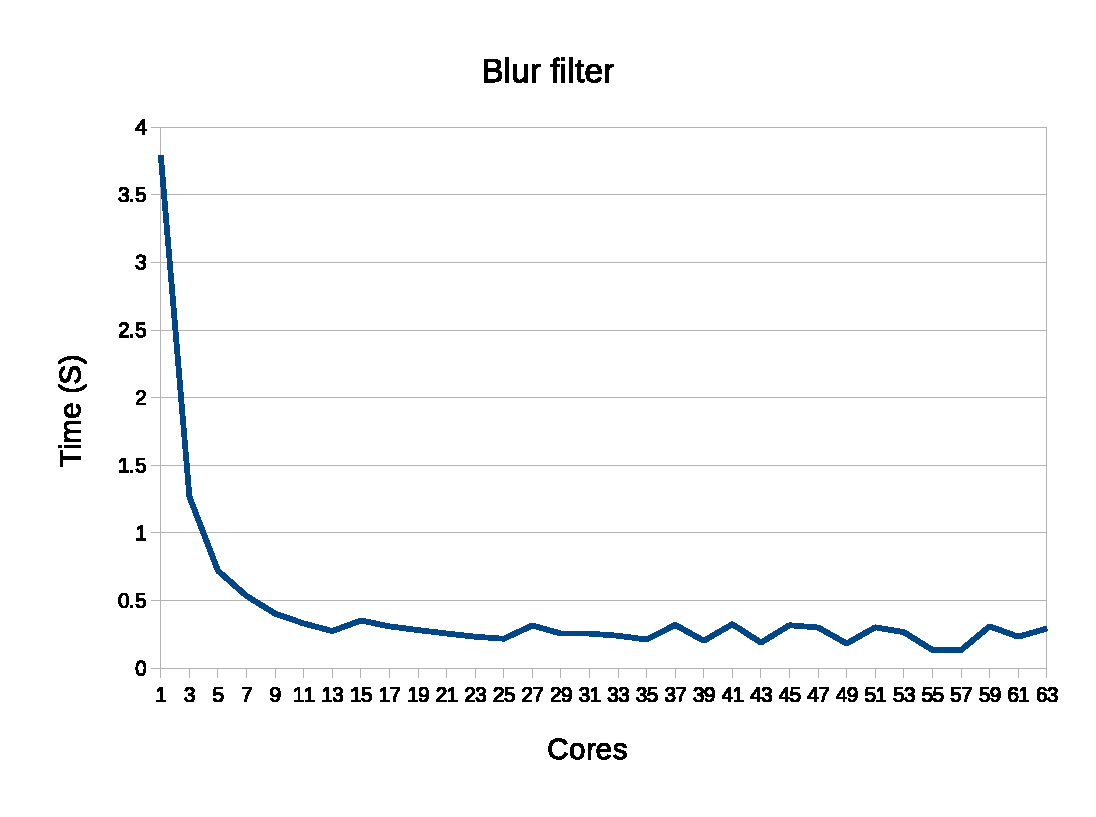
\includegraphics[scale=0.4]{figurer/blur.eps}
	\end{center}
	\caption{Times for blur filter with radius 21}
\end{figure}

\section{Result}
\begin{figure}[H]
	\begin{center}
		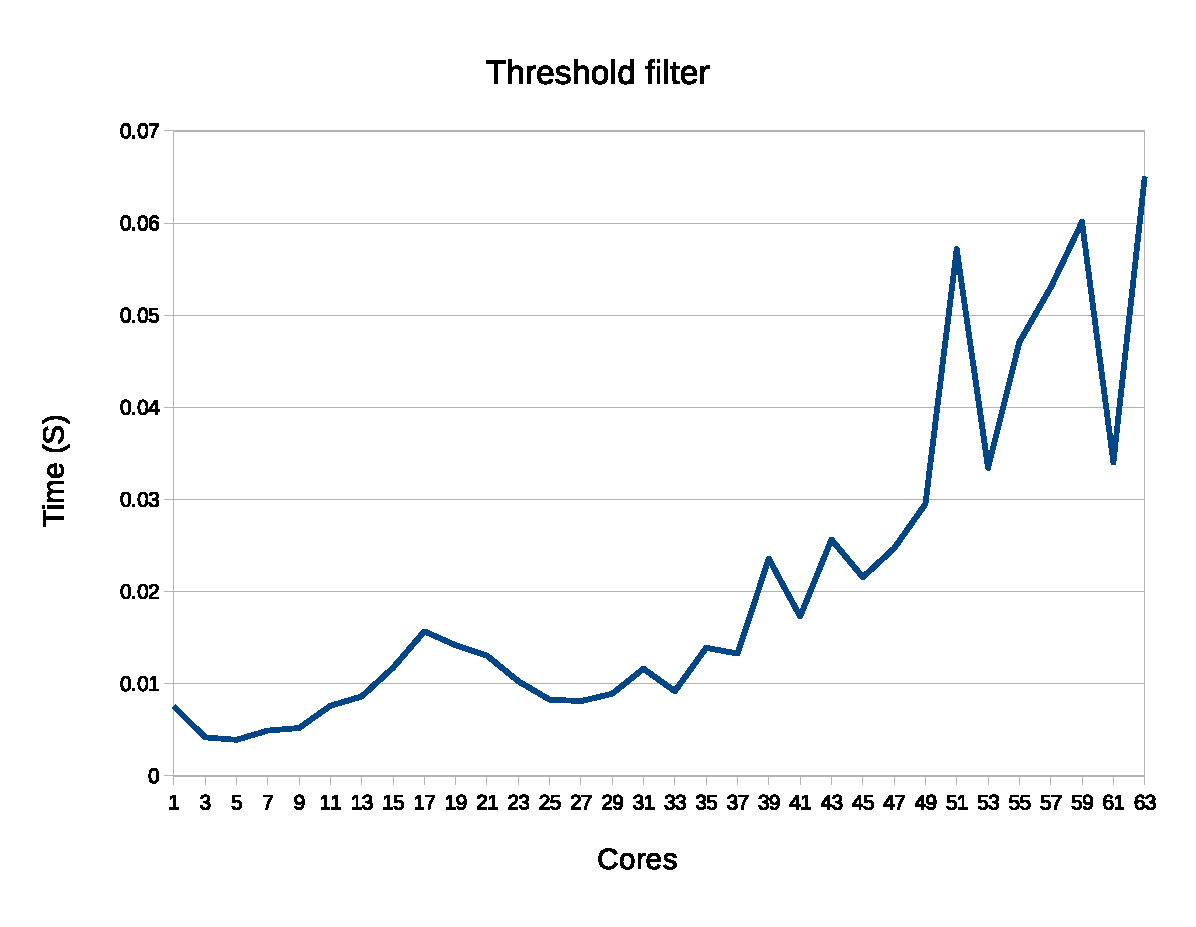
\includegraphics[scale=0.4]{figurer/thres.eps}
	\end{center}
	\caption{Times for threshold filter}
\end{figure}

\newpage

\onecolumn
\appendix
\section{blurmainmpi.c} \label{app:blur}
\lstinputlisting[language=c]{../blurmainmpi.c}

\section{thresfiltermpi.c} \label{app:blur}
\lstinputlisting[language=c]{../thresfiltermpi.c}

\end{document}
